% Figure 1 composite assembly (vector-preserving) for AllelePerturb.
% 6 panels: a pipeline (measurement->model->evaluation->verdict + single-cell
% resolution diagnostic; subsumes old workflow g), b tracks+legend, c depth,
% d features+PCA, e evaluation, f splits. Build: pdflatex fig1_assemble.tex.
\documentclass[tikz,border=1mm]{standalone}
\usepackage{graphicx}
\usepackage{helvet}
\renewcommand{\familydefault}{\sfdefault}
\begin{document}
\begin{tikzpicture}[x=1mm,y=1mm]
  \useasboundingbox (0,31) rectangle (183,202);

  % ---------- Row 1: a (pipeline, 3:2 wide) | b (variant tracks + legend) -------
  % a is 1152x768 pt (3:2); at width 110mm it is 73.3mm tall. b tracks (44mm each)
  % + legend total ~72.6mm so the two panels are bottom-aligned. Height kept close
  % to the previous composite so the Fig.1 float is no worse than before.
  \node[anchor=north west,inner sep=0] at (3,200)   {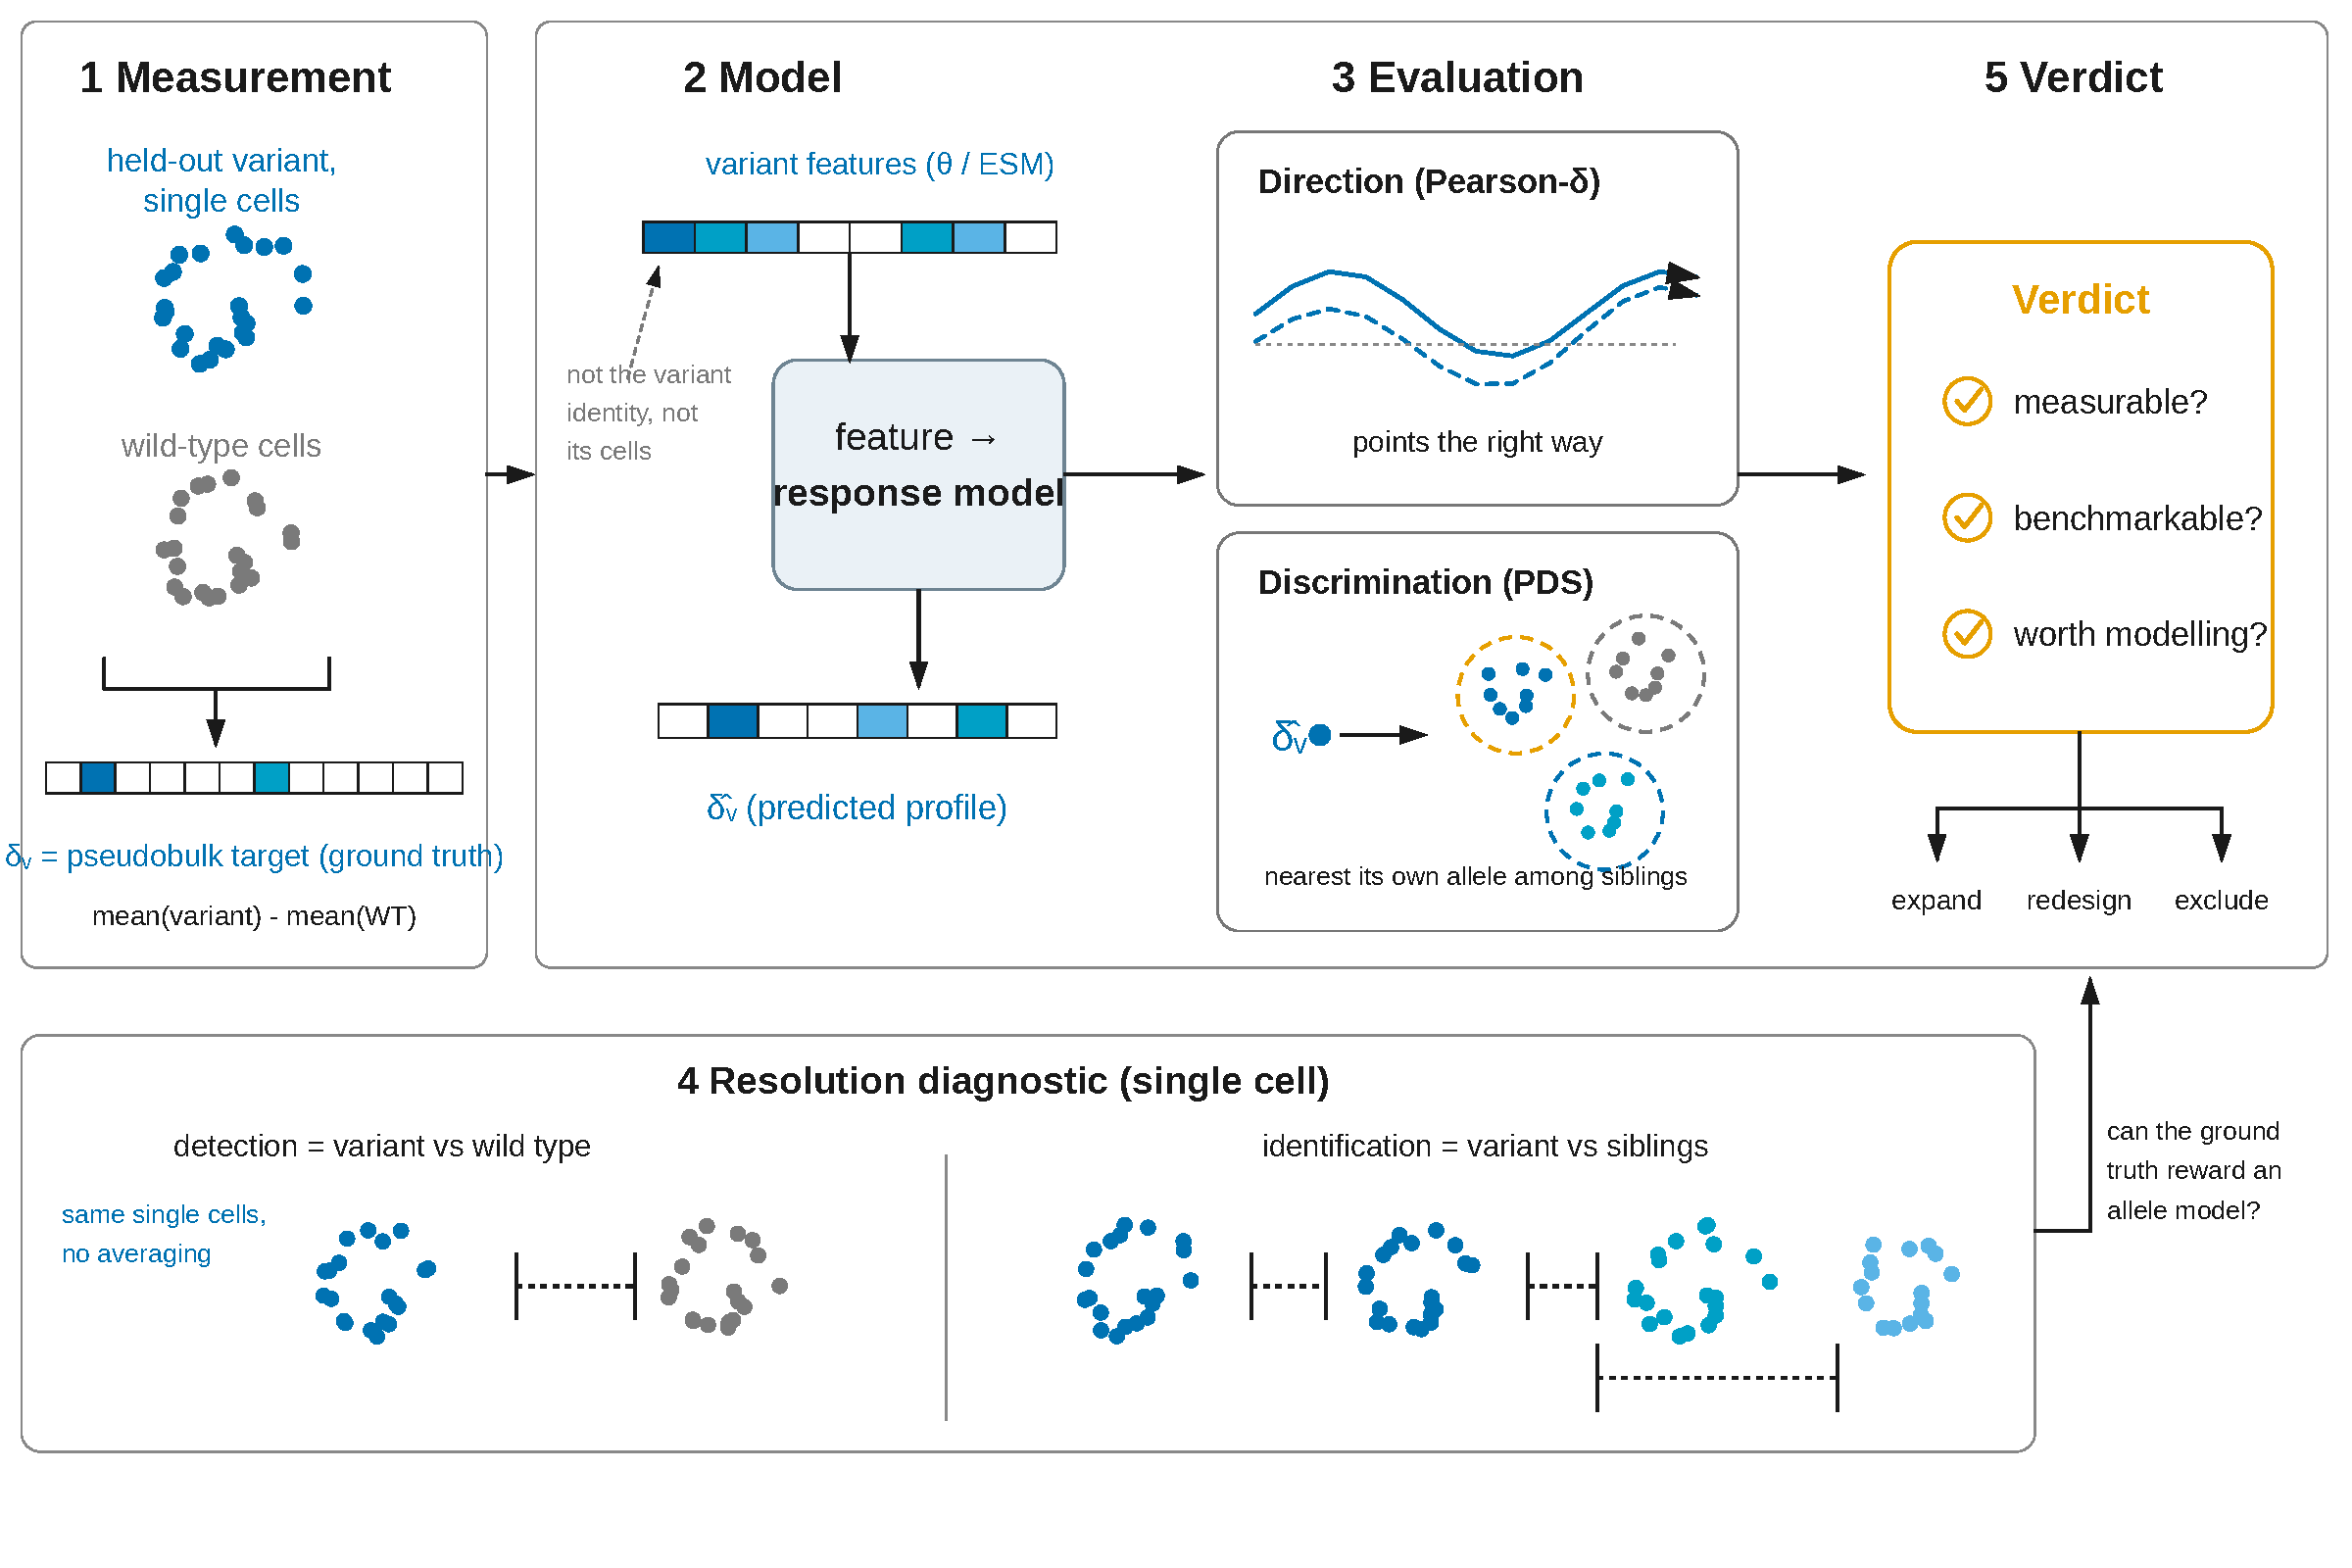
\includegraphics[width=110mm]{Fig1a_editable.pdf}};
  \node[anchor=north west,inner sep=0] at (126,200)
    {\begin{minipage}{44mm}
       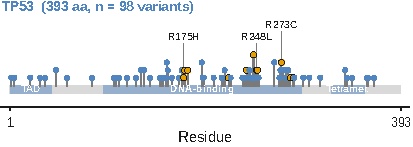
\includegraphics[width=\linewidth]{fig1b_track_TP53.pdf}\\[-0.3mm]
       
\includegraphics[width=\linewidth]{fig1b_track_KRAS.pdf}\\[-0.3mm]
       
\includegraphics[width=\linewidth]{fig1b_track_GATA1.pdf}\\[-0.3mm]
       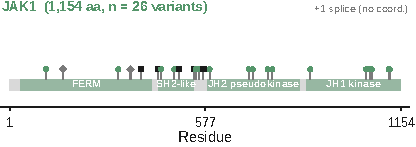
\includegraphics[width=\linewidth]{fig1b_track_JAK1.pdf}\\[0.4mm]
       \hspace*{5mm}
\includegraphics[width=32mm]{fig1b_legend.pdf}
     \end{minipage}};

  % ---------- Row 2: c (depth) | d (features + PCA inset) | e (evaluation) ------
  \node[anchor=north west,inner sep=0] at (3,123)   {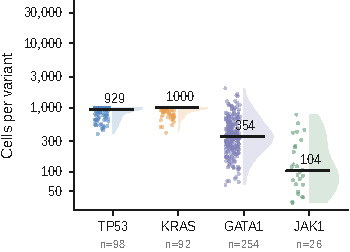
\includegraphics[width=48mm]{fig1c_depth.pdf}};
  \node[anchor=north west,inner sep=0] at (54,123)  {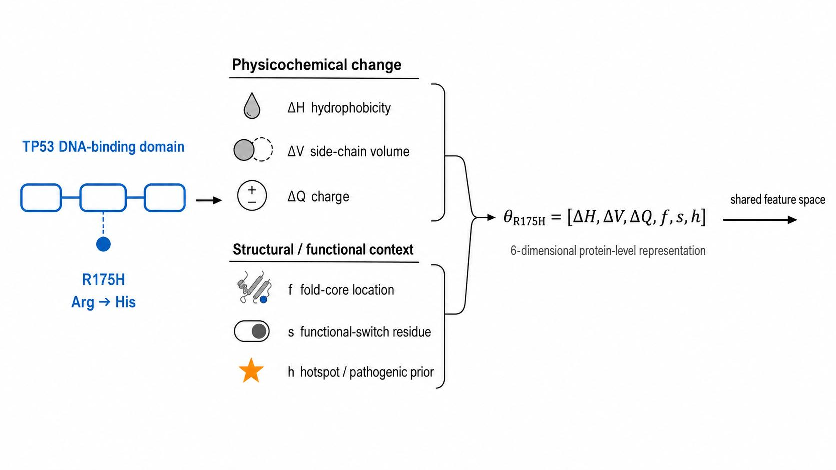
\includegraphics[width=58mm]{Fig1d_schematic_highres.pdf}};
  \node[anchor=north west,inner sep=0] at (89,117)  {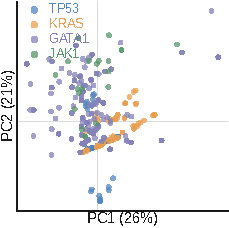
\includegraphics[width=19mm]{fig1d_theta_pca.pdf}};
  \node[anchor=north west,inner sep=0] at (117,123) {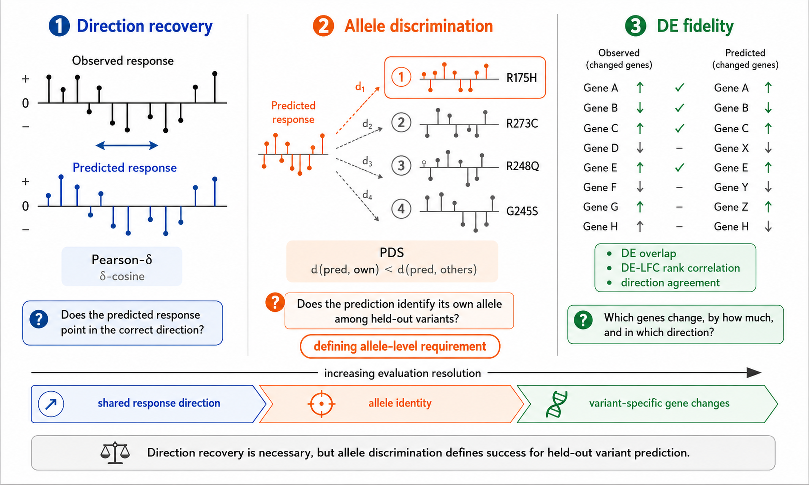
\includegraphics[width=52mm]{Fig1e_Eval_highres.pdf}};

  % ---------- Row 3: f (six generalization splits), centred --------------------
  \node[anchor=north west,inner sep=0] at (51,84)   {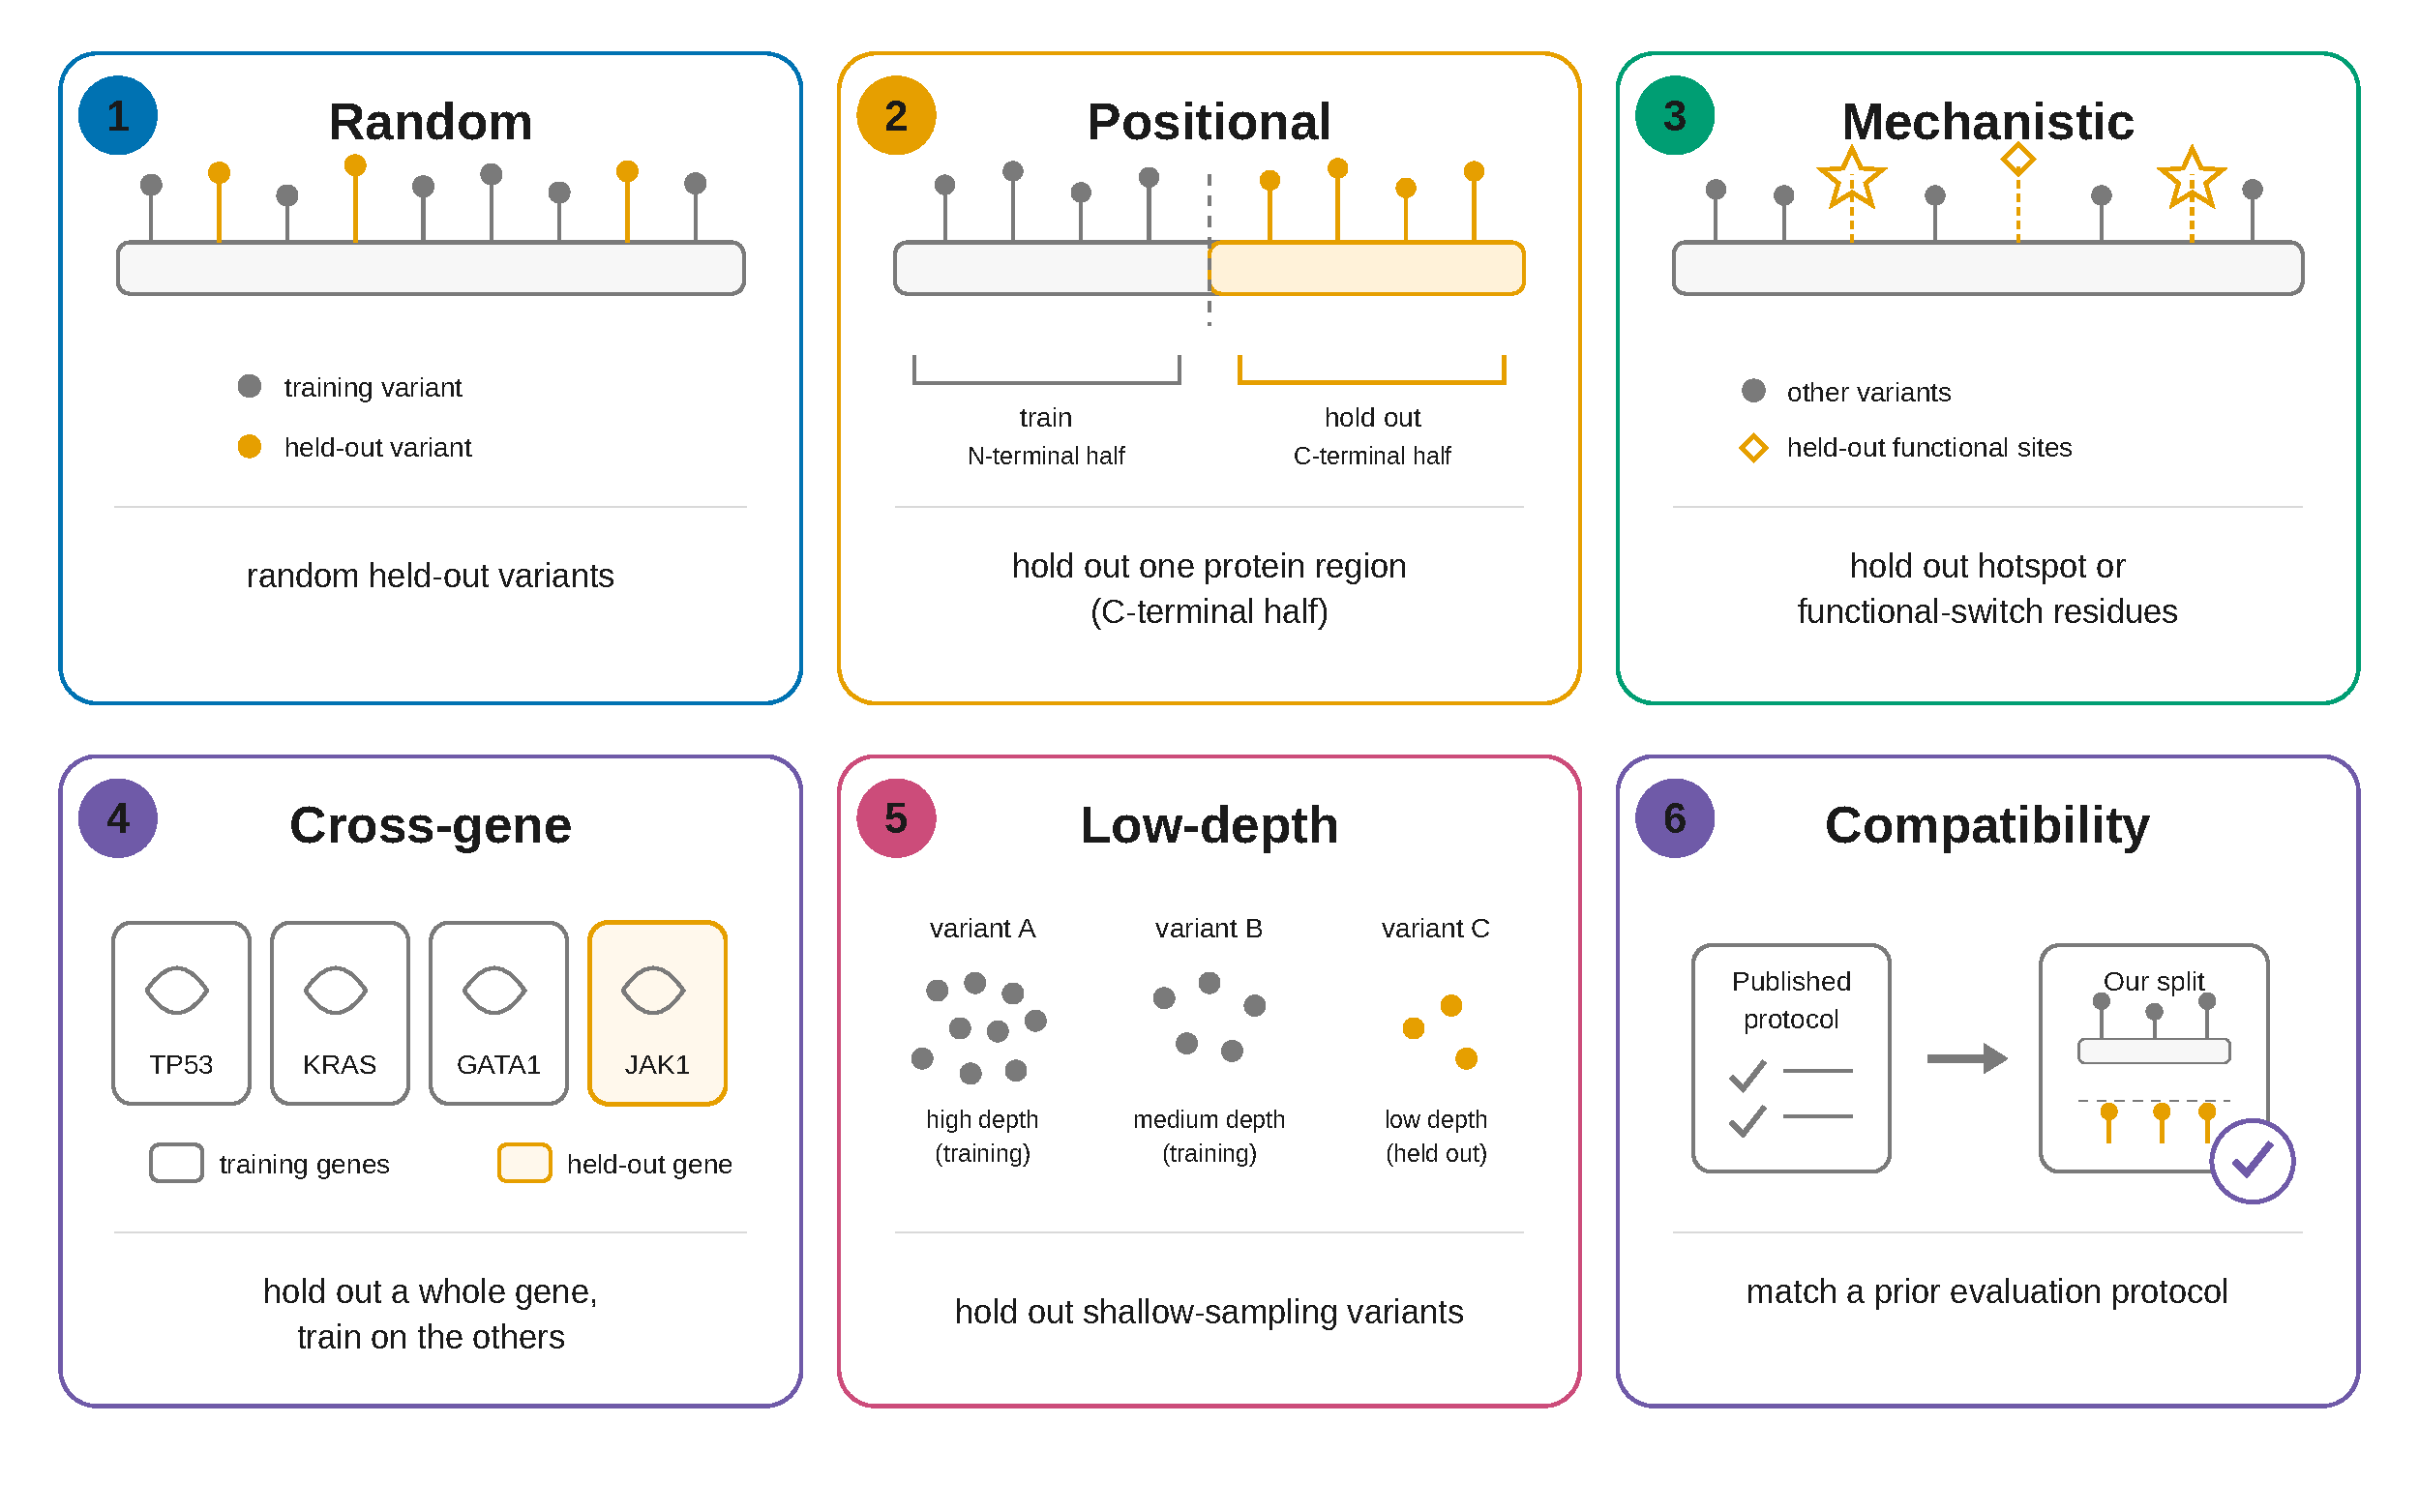
\includegraphics[width=78mm]{Fig1f.pdf}};

  % ---------- panel letters ----------------------------------------------------
  \tikzset{plab/.style={font=\bfseries\large,anchor=north west,inner sep=0}}
  \node[plab] at (1,201.5) {a};
  \node[plab] at (124,201.5) {b};
  \node[plab] at (1,122.5) {c};
  \node[plab] at (52,122.5) {d};
  \node[plab] at (115,122.5) {e};
  \node[plab] at (49,85.5) {f};
\end{tikzpicture}
\end{document}
